\chapter{短波语音客观质量评价算法}
\label{chap:algorithms}

为了能够从多路短波语音中自动切换选择,需要使用算法对各路短波语音的质量进行评价。由于系统没有原始语音作为参考,所以需要的客观质量评价算法是单端的客观评价算法。现有的语音客观质量评价算法主要针对VoIP应用、语音编解码系统、语音降噪系统等场景,这些场景中的语音质量相较短波语音要好,信噪比较高。直接将现有的算法应用到短波语音上难以取得良好的评价结果。所以本章提出了两种可用在短波语音上的客观质量评价算法

\section{基于语谱图噪音模型的客观质量评价算法}

\subsection{启发性思路}

语谱图是一种从频域对语音信号进行分析的工具,将语音信号转换到频域进行分析,需要使用短时傅里叶变换(STFT)。给定一个时间宽度很短的窗函数,语音信号的STFT定义为\ref{eq:stft}

\begin{equation}\label{eq:stft}
F_{STFT}(t, f) = \int_{-\infty}^{+\infty}x(u)g^*(u-t)e^{-j2\pi fu}du
\end{equation}

由于窗函数在时域有限,使得短时傅里叶变换具有局部特性,能够反映指定时刻的局部频谱信息。
实际应用中,需要使用离散化的短时傅里叶变换,取$t=mT, f=nF$,其中$T$和$F$分别为时间和频率的采样间隔,$m,n=0,1,2,...,M-1$,$M$是采样点数。则离散形式的STFT为\ref{eq:dstft}

\begin{equation}\label{eq:dstft}
F_{STFT}(m, n) = \sum_{k=0}^{N-1}x(kT)g^*((k-m)T)e^{-j2\pi nk/N}
\end{equation}

$F_{STFT}(m, n)$反映的是$mT$时刻,$nF$频率附近的局部频谱信息。

根据对于人耳听觉特性的一些研究,人耳对于声音信号的相位特性并不敏感,但是对于幅度特性敏感,并且人耳对于声音响度的感受是与信号能量的对数成正比的。所以对离散短时傅里叶变换得到的结果,只保留幅值能量,并进一步做取对数的处理,得到的二维信息可以用图像展示,称之为语谱图,定义为\ref{eq:log_dstft}

\begin{equation}\label{eq:log_dstft}
G(m, n) = log(|F_{STFT}(m, n)|^2)
\end{equation}

语谱图反映了语音信号在不同时间、不同频率上的能量大小,承载了语音所包含的信息。高质量语音的语谱图上有着清晰的结构特征,包括基音部分的能带,各种高次谐波的能带;而带有噪音的语谱图则没有模糊不清。在短波语音信号上亦是如此。如图~\ref{fig:timefreq}所示,从左到右是质量由低到高五组短波语音的语谱图,分别对应主观评分1-5分。从语谱图上可以看到条带状的语音部分越来越突出和明显。图~\ref{fig:timefreq-thr0.3}是由图~\ref{fig:timefreq}中各个语谱图以0.3为阈值转化为二值图像的结果,图中可以更加明显的看出质量越好的语音信号,条带状的纯净语音部分越清楚,而质量较差的语音信号,则因为存在噪音连成模糊的一片。

\begin{figure}
\centering
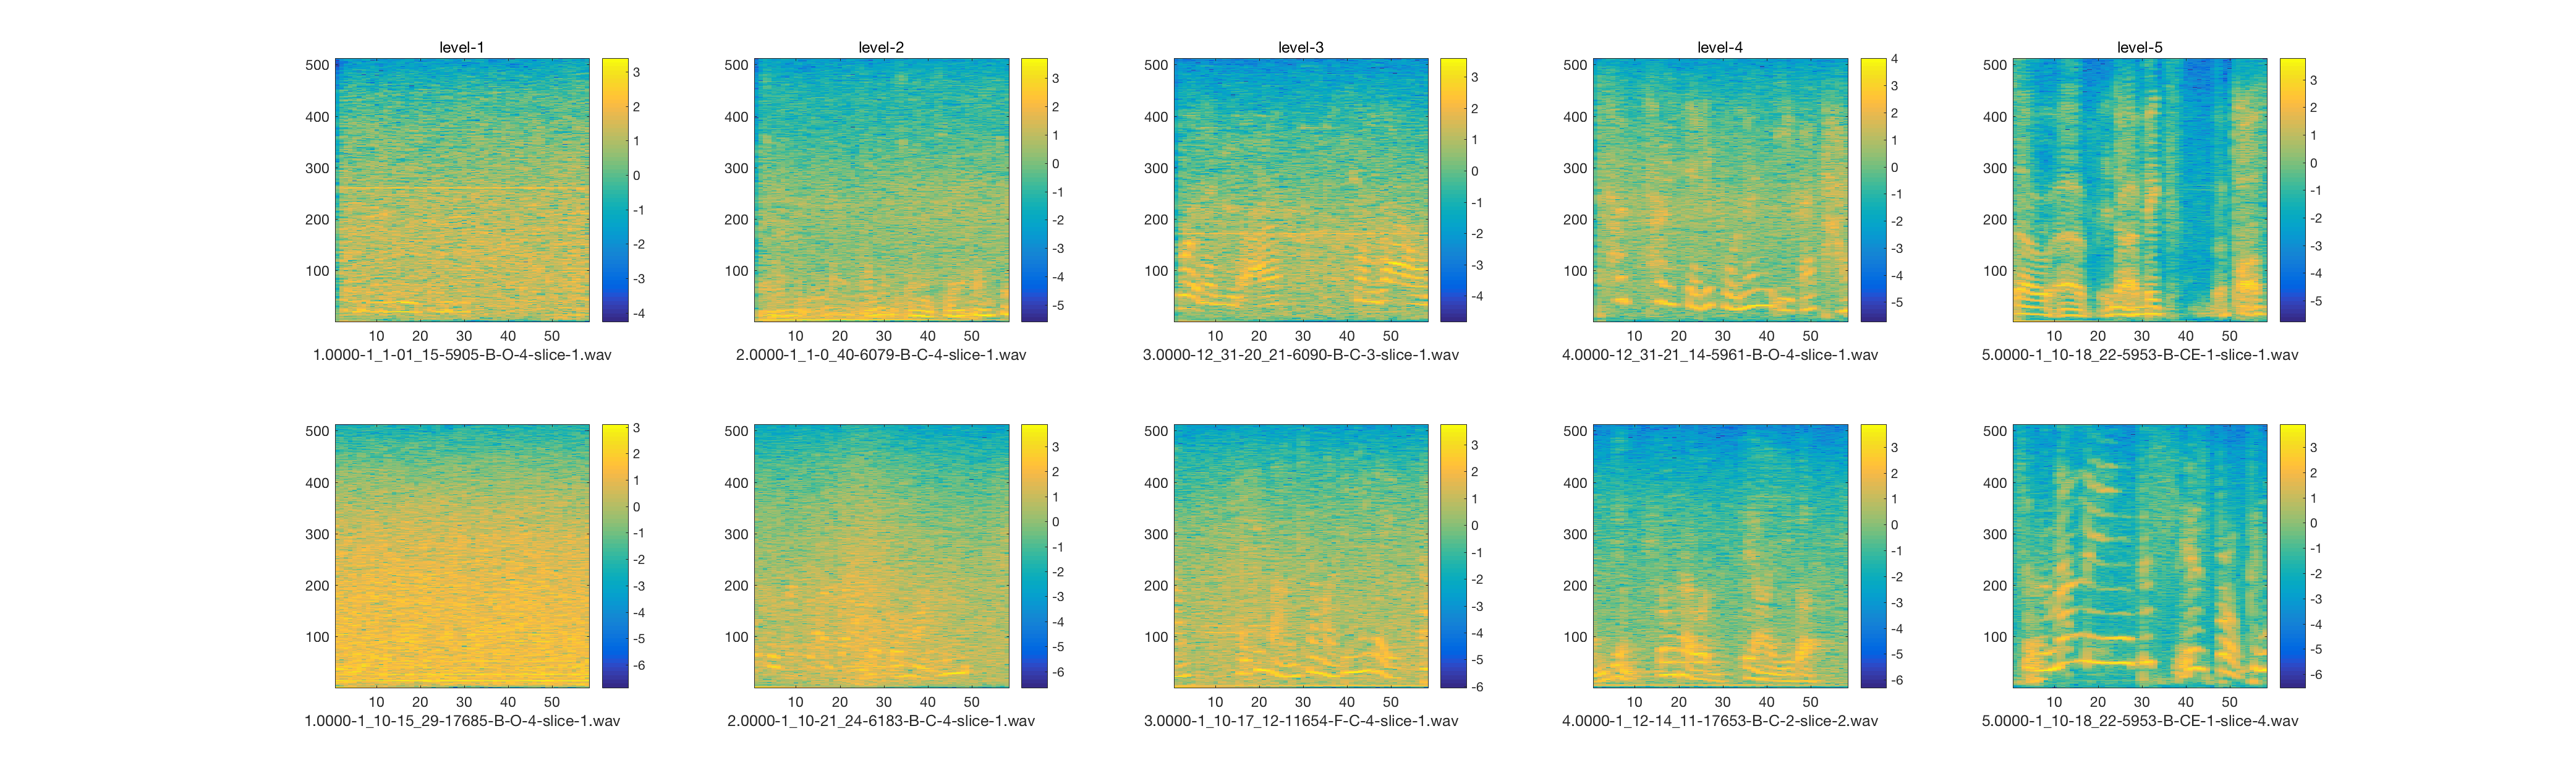
\includegraphics[width=1\textwidth]{timefreq}
\caption{不同质量的短波语音语谱图\label{fig:timefreq}}
\end{figure}

\begin{figure}
\centering
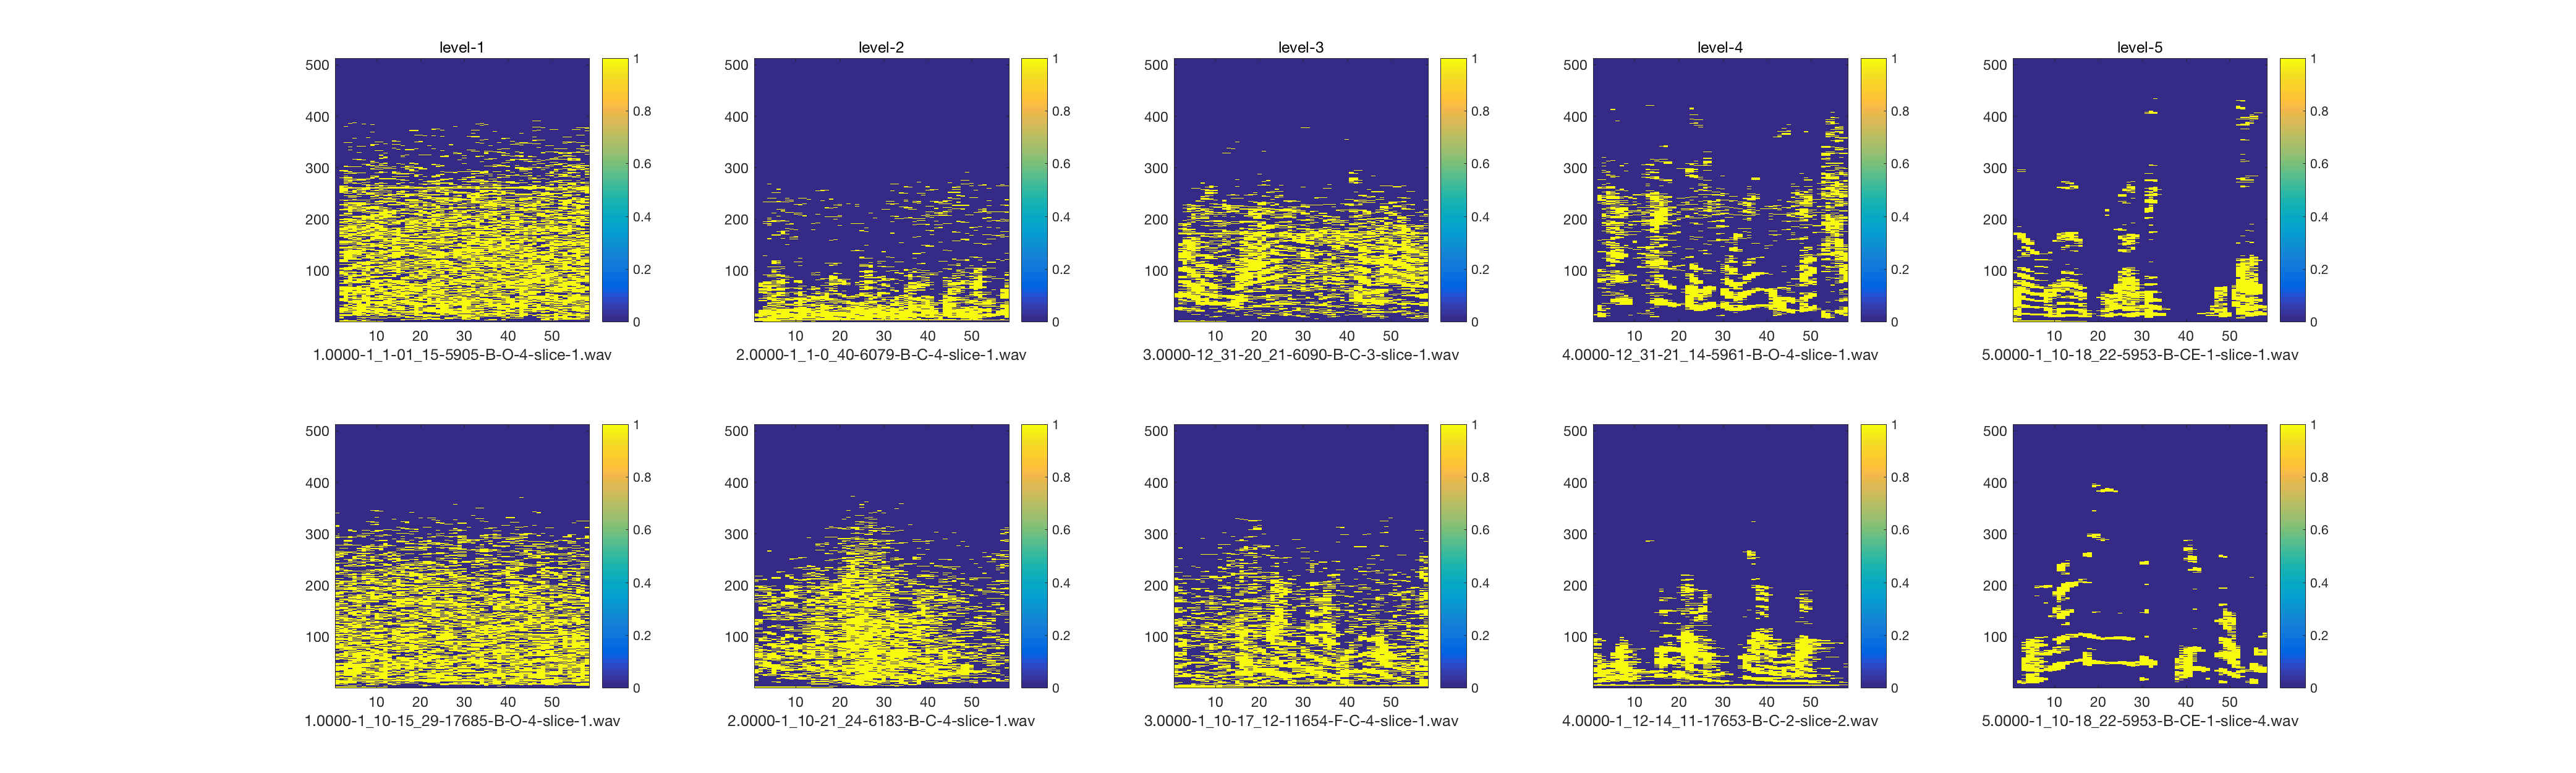
\includegraphics[width=1\textwidth]{timefreq-thr}
\caption{不同质量的短波语音二值化语谱图\label{fig:timefreq-thr0.3}}
\end{figure}

\begin{figure}
\centering
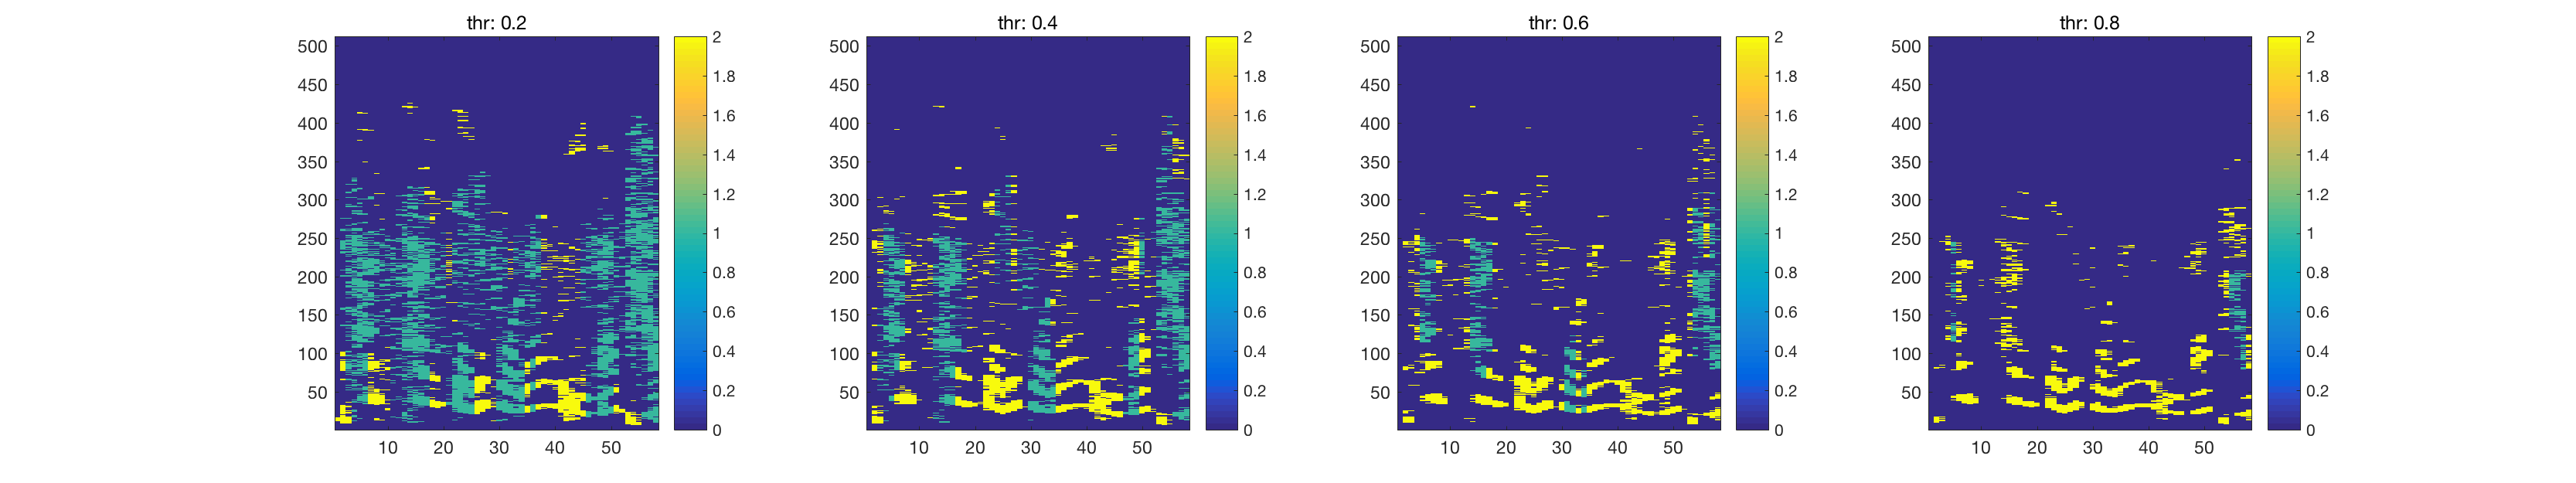
\includegraphics[width=1\textwidth]{timefreq-thrs-label}
\caption{不同阈值的二值化语谱图\label{fig:timefreq-thrs-label}}
\end{figure}

进一步地,从中选出一个语音信号,分别以0.2, 0.4, 0.6, 0.8为阈值绘制其二值化语谱图,如图~\ref{fig:timefreq-thrs-label}所示。而图中绿色区域是程序通过建立噪音模型,使用一些特征标注出的被噪音干扰的区域。可以发现,在阈值较低时,因为噪音部分留在了图上,所以看上去是大片大片的噪音;而当阈值逐渐升高,噪音部分逐渐从图上消失,留下的就都是纯净的语音信号。若当阈值超过某一阈值t时,语谱图上某一点不再被噪音干扰,那么这一点实际能量比t高出的部分就表征了这一点语音信号相对于噪音部分高出的强度。本文称之为该点的语音分辨率,计算语谱图上所有点的语音分辨率,进而得出语音质量的客观评价分。

\subsection{算法流程}

本小节介绍基于语谱图噪音模型的客观质量评价算法的具体流程,算法总体流程示意如图~\ref{fig:flowchart}所示。一维的短波语音信号经过加窗傅里叶变换得到二维的频域信号,其中横轴为时间维度,纵轴为频率维度。随后用不同阈值将语谱图转化成多张二值图像,再各个二值图像上使用图像处理的一些方法区分噪音区域和语音区域。再此基础上得到原始语谱图上各个点的“语音分辨率”,进而得到对于短波语音的客观评价分数。下面详细介绍各个步骤的内容。

\begin{figure}
\centering
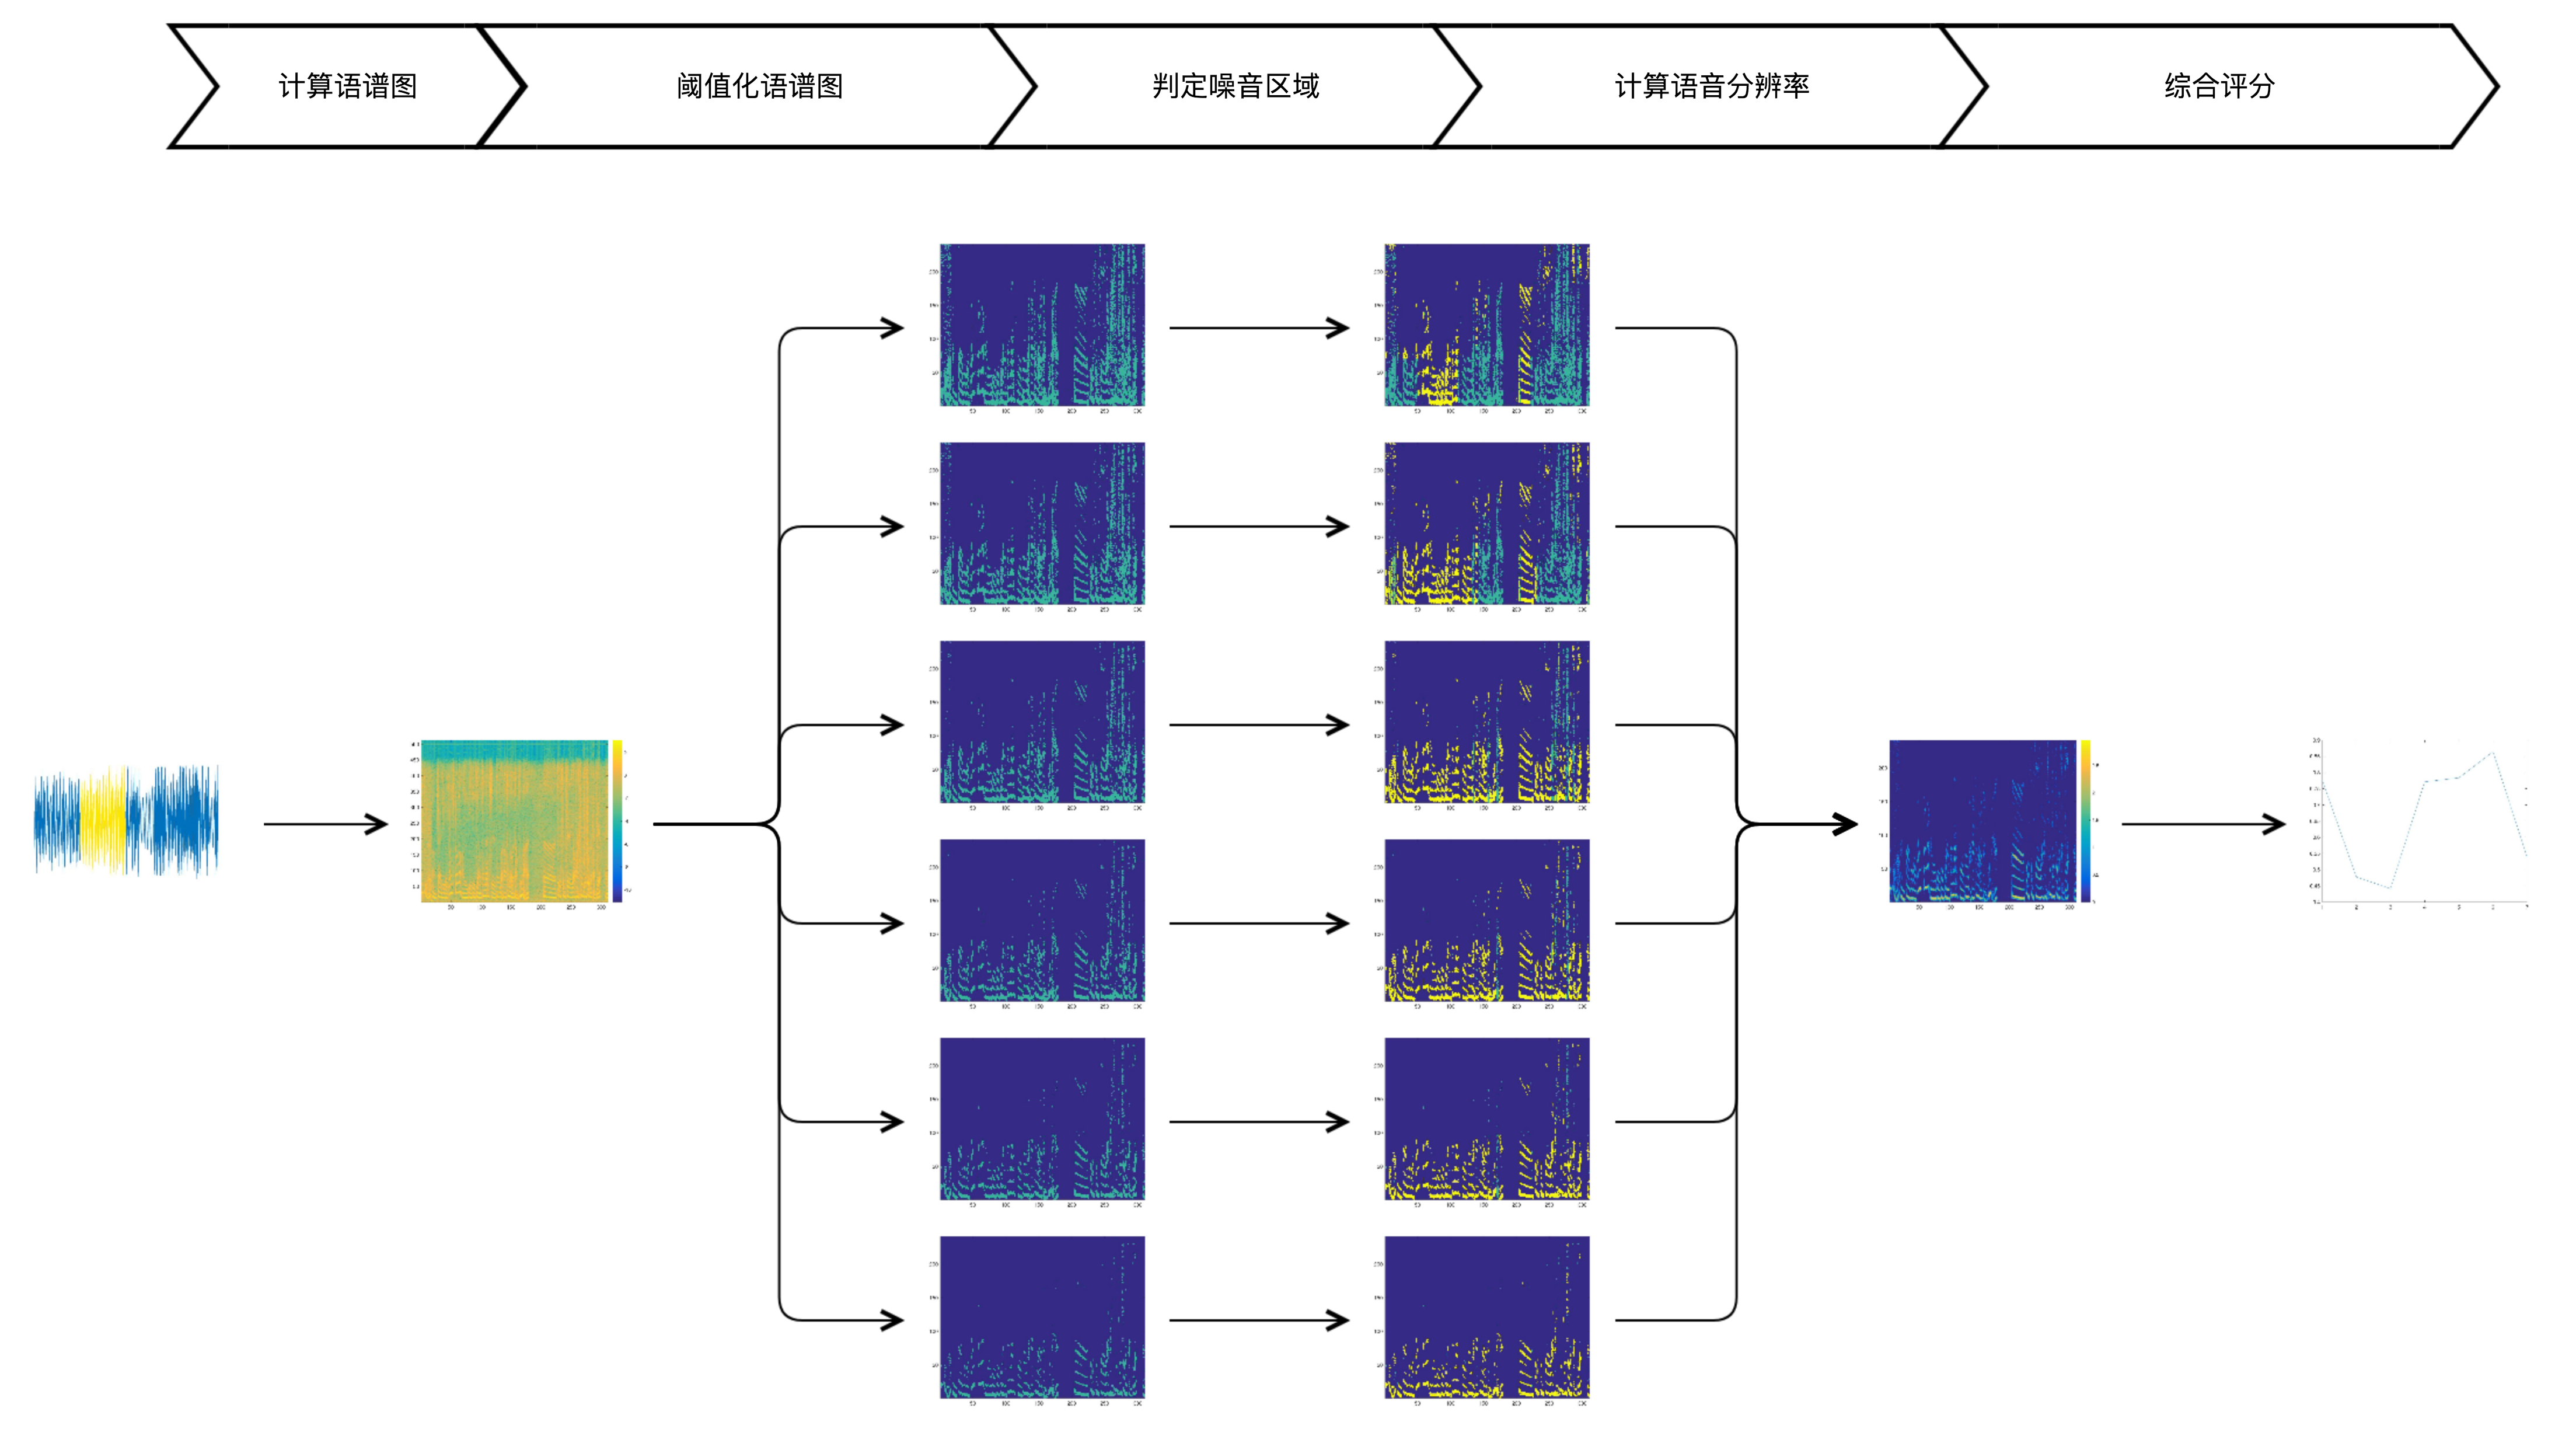
\includegraphics[width=0.8\textwidth]{flowchart}
\caption{基于语谱图噪音模型的客观质量评价算法流程\label{fig:flowchart}}
\end{figure}

首先根据上一小节介绍的语谱图的内容,使用短时傅里叶变换获得短波语音信号的语谱图$G(m,n)$。

取一系列的阈值$t_1<t_2<t_3<...<t_N$,我们进一步对语谱图做阈值化处理形成二值的语谱图,阈值化语谱图定义为

\begin{equation}\label{eq:thr_tf}
G_i(m, n) = \left\{
    \begin{array}{rcl}
    1, && {G(m,n)>t_i} \\
    0, && {G(m,n)\leq t_i}
    \end{array} \right.
\end{equation}

根据短波语音语谱图上的噪音模型,使用以下几种条件来判定噪音区域:
\begin{enumerate}
\item 区域$A_1$:语谱图上通过霍夫变换检测的与水平夹角小于1度的直线。
\item 区域$A_2$:某一长宽各大于一定阈值的范围内,$G_i(m,n)=1$的点数占据面积的80\%以上。
\item 区域$A_3$:某一连通域面积比上该连通域占据的宽度,其值超过一定阈值。
\item 区域$A_4$:某一连通域,其面积小于一定阈值。
\end{enumerate}

标注后的语谱图
\begin{equation}\label{eq:label_tf}
G_i^*(m, n) = \left\{
    \begin{array}{rcl}
    0, && {G_i(m,n)=0} \\
    1, && {G_i(m,n)=1且(m,n)\in \bigcup_{k=1}^4 A_k} \\
    2, && {else}
    \end{array} \right.
\end{equation}

定义集合
\begin{equation}\label{eq:collection}
\Psi(m,n)={i|G_i*(m,n)=2}
\end{equation}

定义语音分辨率
\begin{equation}\label{eq:resolution}
D(m,n) =  \left\{
    \begin{array}{rcl}
    0, && {\Psi(m,n)=\emptyset} \\
    G(m,n) - \min_{i\in\Psi(m,n)}t_i, && {\Psi(m,n)\neq\emptyset}
    \end{array} \right.
\end{equation}

对语音分辨率取平均得到客观评价分数
\begin{equation}\label{eq:score}
S = \frac{\sum D(m,n)}{\sum G_1(m,n)}
\end{equation}

为保证阈值化语谱图包含有效信息,阈值参数的取值范围应该是。一种简单的选取方法是直接在到选取$N$等分点。
为了尽量细致地刻画语谱图的特征,阈值的选取应该尽量密集,但同时算法的时间复杂度正比于阈值的数量,密集的阈值也会导致更高的计算复杂度。所以阈值的选取应当使用尽量少的阈值尽量高效地刻画语谱图的特征,上述选取方法显然不够高效。一方面,阈值很接近$\min{G(m,n)}$或者$\max{G(m,n)}$时,阈值化语谱图上的点非常少或者非常多,能提供的信息量很少。另一方面因为阈值增加同样大小,阈值化语谱图上的点数增加可能差异很大。均匀地选取阈值,会导致在有些区间,连续的几张阈值化语谱图过于相像而浪费计算资源,有些区间,阈值化语谱图又变化太快导致刻画不够细致。

一种改进的动态选取阈值的方法如下:先在5\%至20\%之间均匀选定一系列比例$\alpha_1,\alpha_2,\alpha_3,...,\alpha_N$,再计算得出对应的阈值$t_1,t_2,t_3,...,t_N$使得$\sum G_i(m,n)=\alpha_i M^2$。实验验证此种阈值选取方法要比前述方法效果提升很多。


\section{基于自编码器的客观质量评价算法}

上节介绍的基于语谱图噪音模型的客观质量评价算法虽然能够很好的评价短波语音的质量,实验也表明算法给出的评分能够反映人的主观感受。但是该算法是基于人为经验分析的语谱图噪音模型,在应用到其他领域的低信噪比语音时,由于可能存在的噪音不一样,需要重新分析噪音的模型特征。所以该算法针对性很强,而适用性则较窄,迁移应用较难。

为此,本节从另一个角度出发,通过人工神经网络的自编码器学习纯净短波语音的语谱特征,对语音部分而非噪音部分建模,然后再使用自编码器来评价短波语音的质量。由于人工神经网络的学习可以自动完成,不需要过多人工干预,所以这种方法可以方便的迁移到其他领域的应用中。

